\documentclass{article}
\usepackage{amsmath}
\usepackage{mathtext}
\usepackage[english,russian]{babel}
\usepackage[T2A]{fontenc}
\usepackage[utf8]{inputenc}
\usepackage{graphicx}
\graphicspath{{img/}}
\DeclareGraphicsExtensions{.jpg, .png, .pdf}
\begin{document}
\section{Сложные передачи. Волновые передачи.}

По конструктивному исполнению различают фрикцонные и зубчатые. Р-м принцип действия фрикционной влонвой передачи

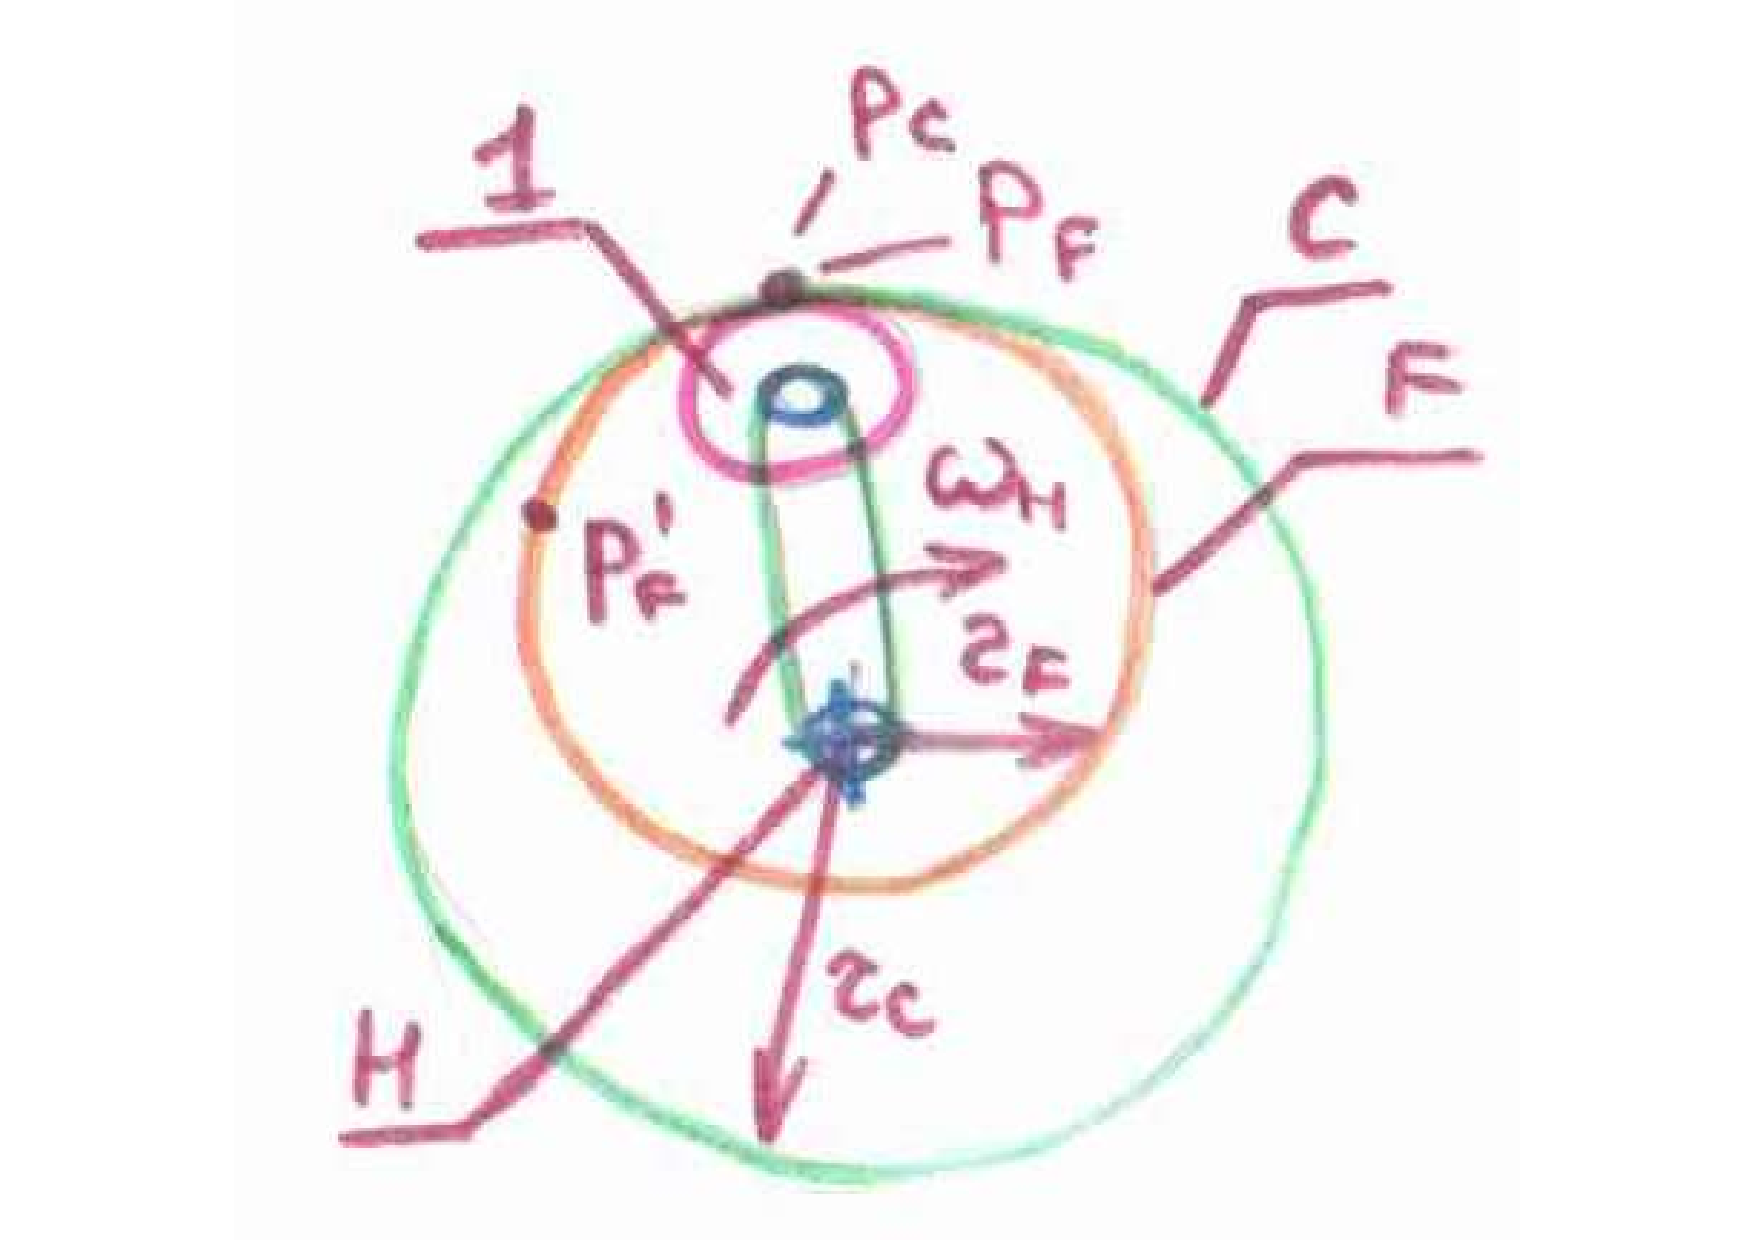
\includegraphics[width = \textwidth]{1}

Внутрь жесткого неподвижного цилиндрического кольца C вставлено гибкое кольцо F? прижатое роликом 1, закрепленным на водиле H
$L_F$ -- длина внутренней окр-ти.
$L_C$ -- длина внешней окр-ти.

При вращении водила по часовой стрелке, внутреннее колесо вращается против часовой стрелки. Считаем, что проскальзывание отсутствует.

За 1 оборот водила гибкое кольцо повернется на небольшой угол, определяемый дугой $\rho_F$ $\rho_F^{'} = L_C - L_F$, посему чем меньше разница длины окружностей, тем меньшеугол поворота внутреннего колеса.

Таким образом, происходит преобразование быстрого вращения водила с угловой скоростью $\omega_H$ в обратное по направлению и замедленное по вражению гибкого вала кольца

$$
i_{HF} = \frac{L_F}{L_C - L_F}  = - \frac{\pi dc}{\pi dc - \pi df} = - \frac{dF}{ \Delta} 
$$
$$
i_{HF} = - \frac{z_F}{z_C - z_F} 
$$

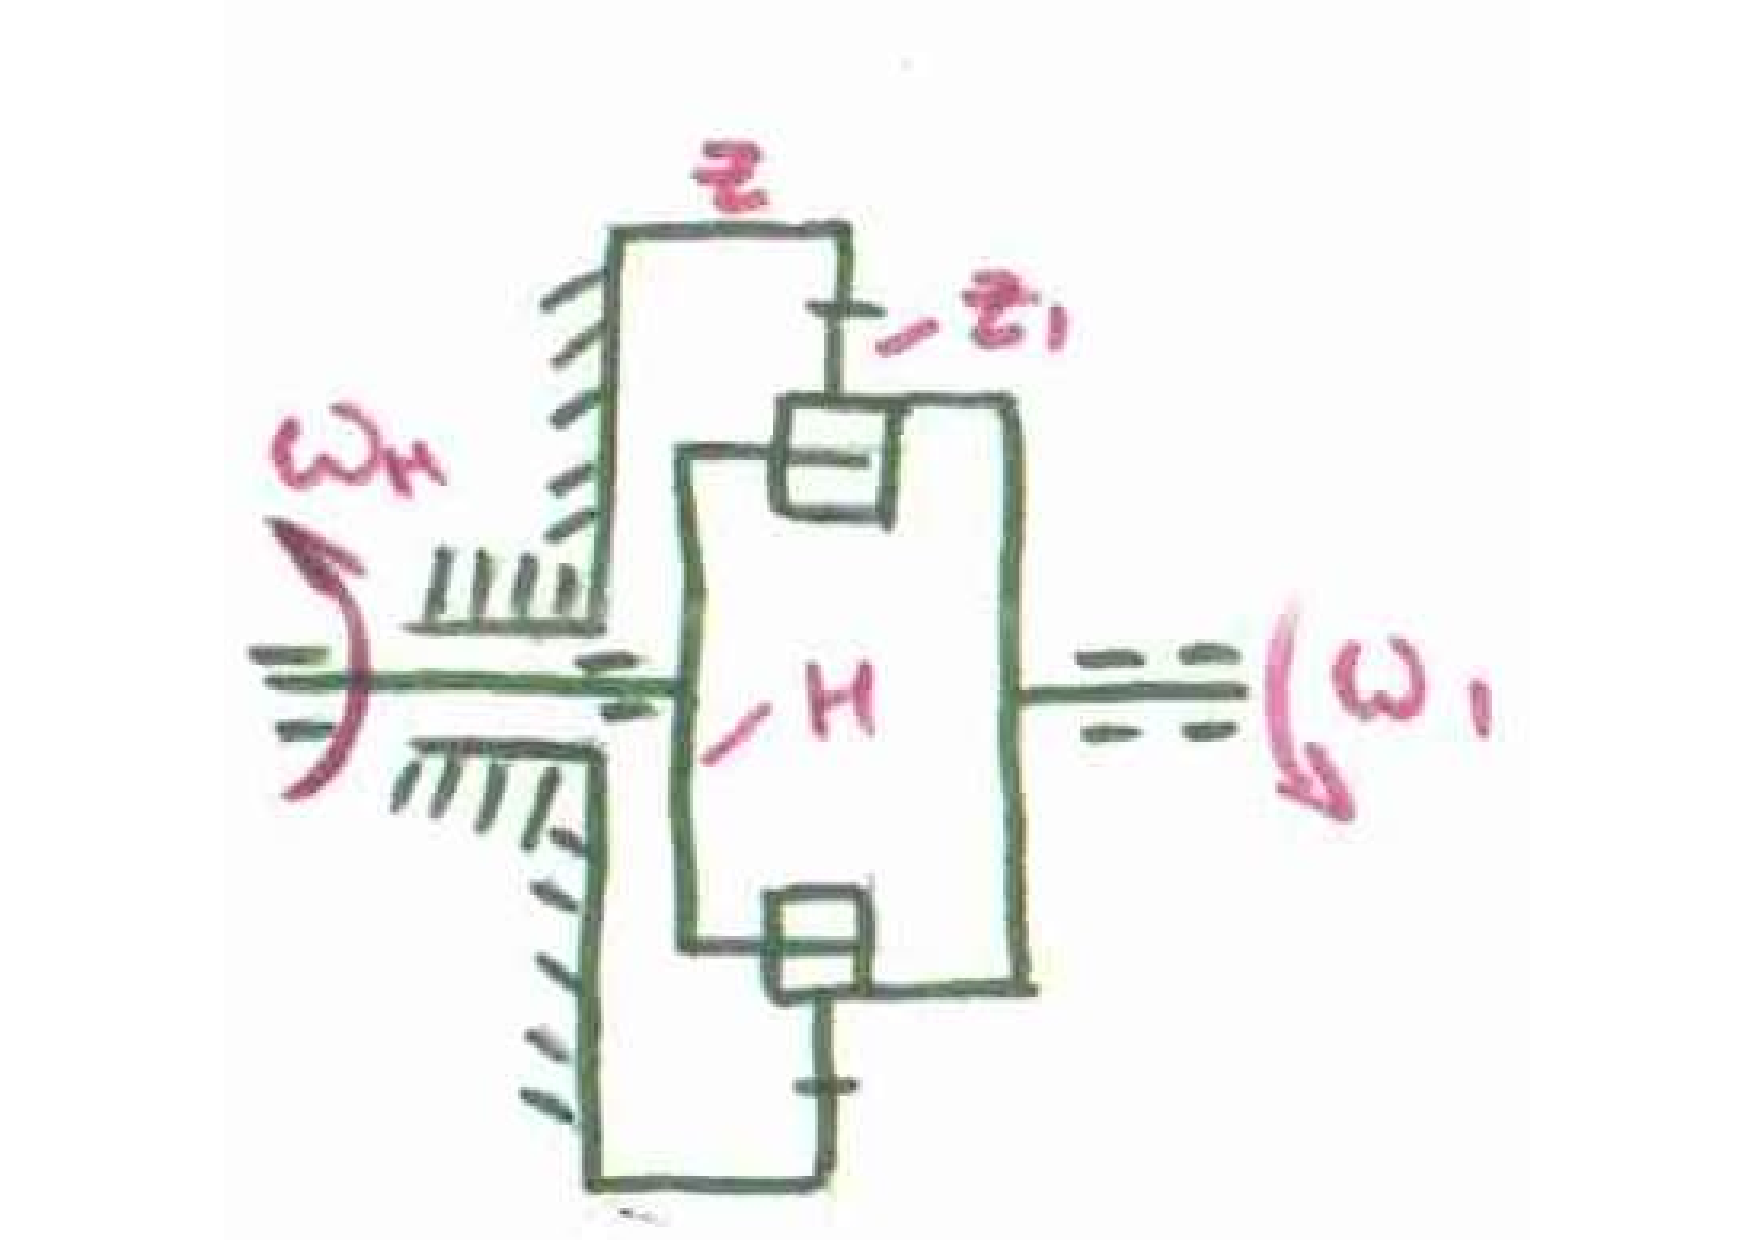
\includegraphics[width = \textwidth]{2}

\underline{Достоинства} 
\begin{enumerate}
	\item Выскоая нагрузочная способность т.к. в закцеплении всегда находятся 30-50\% зубьев
	\item Более высокая кинематическая точность в сравнии с обычными зумбчатыми редукторами, т.к большое кол-во зубьев одновеменно находятся в зацеплении и погрешность окружных шагов устраняется
	\item Работает сравнительно плавно и бесшумно
	\item $\eta = 80 .. 90 \%$
	\item Возможность передачи движения через герметичную стенку
\end{enumerate}
\underline{Недостатки}
\begin{enumerate}
	\item Специфические материалы гибкого колеса быстро изнашиваются
\end{enumerate}
\end{document}
